% --------------------------------------------------------------
% This is all preamble stuff that you don't have to worry about.
% Head down to where it says "Start here" % --------------------------------------------------------------
 
\documentclass[12pt]{article}

\usepackage{listings}
\usepackage[margin=1in]{geometry} 
\usepackage{amsmath,amsthm,amssymb}
\usepackage{graphicx}
\usepackage{hyperref}
\graphicspath{ {../} } 

\newcommand{\N}{\mathbb{N}}
\newcommand{\Z}{\mathbb{Z}}
\newcommand\indep{\protect\mathpalette{\protect\independenT}{\perp}}
\def\independenT#1#2{\mathrel{\rlap{$#1#2$}\mkern2mu{#1#2}}}

\newenvironment{theorem}[2][Theorem]{\begin{trivlist}
\item[\hskip \labelsep {\bfseries #1}\hskip \labelsep {\bfseries #2.}]}{\end{trivlist}}
\newenvironment{lemma}[2][Lemma]{\begin{trivlist}
\item[\hskip \labelsep {\bfseries #1}\hskip \labelsep {\bfseries #2.}]}{\end{trivlist}}
\newenvironment{exercise}[2][Exercise]{\begin{trivlist}
\item[\hskip \labelsep {\bfseries #1}\hskip \labelsep {\bfseries #2.}]}{\end{trivlist}}
\newenvironment{reflection}[2][Reflection]{\begin{trivlist}
\item[\hskip \labelsep {\bfseries #1}\hskip \labelsep {\bfseries #2.}]}{\end{trivlist}}
\newenvironment{proposition}[2][Proposition]{\begin{trivlist}
\item[\hskip \labelsep {\bfseries #1}\hskip \labelsep {\bfseries #2.}]}{\end{trivlist}}
\newenvironment{corollary}[2][Corollary]{\begin{trivlist}
\item[\hskip \labelsep {\bfseries #1}\hskip \labelsep {\bfseries #2.}]}{\end{trivlist}}
 
\begin{document}
 
% --------------------------------------------------------------
%                         Start here
% --------------------------------------------------------------
 
%\renewcommand{\qedsymbol}{\filledbox}
 
\title{Assignment 3\\
Big Data Analytics Programming} %if necessary, replace with your course title
\author{Evangelos Ntavelis\\ %replace with your name
r0692337 \\
evangelos.ntavelis@student.kuleuven.be}
 
\maketitle

\tableofcontents

\section{Introduction}
In this assignment we will discuss the performance improvement we can achieve by using indices on database queries and the implementation and performance issues that arise when building a Neighbor-Based Collaborating Filtering System for Movie Recommendations.


\section{Index Structures}

In order to minimize the effect of randomness on the performance of the naive and index based approaches we run the queries one million times, the average time for each query is shown in the Figure \ref{fig:queries}. We also checked that indeed the two queries produce the same results. Let's discuss the results:
\begin{itemize}
    \item \textbf{Queries 1 \& 2:} we observe that the index solution takes 0.9\% and 1.6\% of the naive solution time respectively. The huge improvement makes sense, as when constructed the BitMap we already made the selection, as bits in the attribute columns. Thus selections and their counts are trivial.
    \item \textbf{Query 3:} the use of the BitSlice Index gives us 0.3\% of the naive running time. Comparing with the naive solution here is kind of cheating as the numerical values are stored as Strings we have to parse, a process that is already done for the index. At the same time, the BitSlice structure permits us to easily sum values based on the number of bits we have on each bit column.
    \item \textbf{Query 4:} the fraction here is 4.3\%. We also observe the cumbersome double parsing, yet applying the filter increased the BitSlice index time. 
    \item \textbf{Queries 5 \& 6:} The naive's double parsing here takes less time as it is applied only to a fraction of the records, as the selection happens first. We observe the indices approach to take 22.4\% and 17.4\% of naive's time accordingly.
  \end{itemize}

\begin{figure}[h]
    \centering
    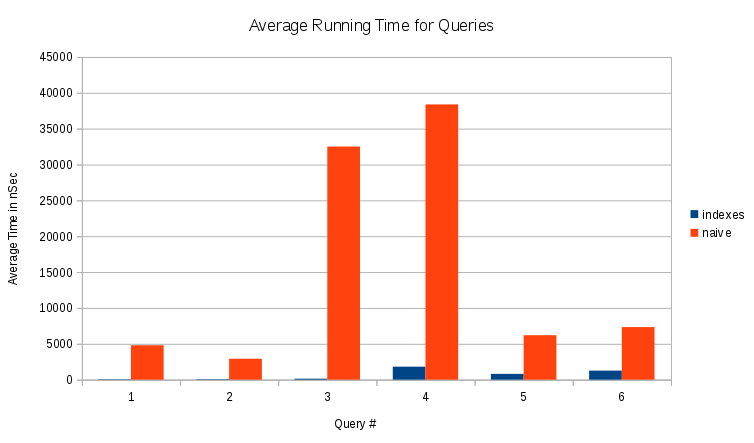
\includegraphics[width=1\textwidth]{queries}
    \caption{Query Performance}
    \label{fig:queries}
\end{figure}
 


\section{Movie Recommendations}

In this part we will describe the decisions we made when implementing the simple Collaborating Filtering model for recommending movies.

\subsection{Fitting the dataset into 2 Gigabytes of RAM}

The first issue we encounter when implementing the model was how to fit the Pearson Correlation Matrix in the limited memory space. Progressively, we found ways to lessen the matrix memory usage:

\begin{itemize}

  \item \textbf{Symmetry:} The Pearson Correlation Formula is symmetrical and so is the corresponding matrix, we could omit storing the diagonal, as we always know that the correlation of an element to itself is 1, and all the values below it.
  \item \textbf{Values Range \& Precision:} The Pearson correlation takes values between -1 and 1; our aim is to store the number rounded to four decimal points. In total we have 20001 numbers, which could fit into a \textit{short} variable type and thus use only 2 bytes per stored correlation.

\end{itemize}

Up to this point we were able to significantly reduce the needed space, but we were not nearly there. Next step, choice of \textbf{Data Structures}. Firstly we developed a wrapper class for user-correlations, afterwards we discovered that the \textit{Neighbors} was a essentially the same idea. Feeling both good and bad with ourselves we adjusted our(?) creation. We also noticed that the most of the Correlation Matrix Values are \textit{NaNs}. 

\begin{itemize}
  \item \textbf{Arrays} Redundantly stores the NaNs and consumes about 5G of RAM
  \item \textbf{Hashmap} At first we used a Hashmap of <Integer, Neighbor>which later upgraded to an Array of Hashmaps <Integer, Correlation>. Both of these implementations consumed more memory than the limit.
  \item \textbf{Arraylists} We ended up using an Array of Arraylists. The problem with this implementation is that the retrieval is not of constant time, which affected the way we implemented the prediction later. 
\end{itemize}

Proud with our ideas, we set to compile and run. The sun out of our window was warmly smiling at us, the sky was the bluest we've encountered the last six months below the eternal gray sky of Belgium. The \textit{outside window} was telling me to go out, the \textit{screen window} was telling me \textit{Memory Error}. So, to further limit our memory usage we made the following choices:

\begin{itemize}
  \item \textbf{Least Common Rated Movies:} the Pearson Correlation formula for 2 items produce only -1 or 1, for 3 we are unable to compute the significance intervals. Generally the less this threshold is, we have more noise in our correlation matrix. We experimented with different values and had the correlation of two user pairs without enough items set to \textit{NaN}.
  \item \textbf{Correlation Threshold:} In Neighbor-Based Collaborating Filtering methods there are two main approaches: set a maximum number of Neighbors or set a minimum threshold to correlation values used for predictions. By setting this limit at the Matrix Computation Stage, we were able to further reduce the usage.

\end{itemize}

At last we made it!

\subsection{Code Performance Choices}

Generally, we tried to omit doing any extra calculations.We made the following note-worthy choices:

\begin{itemize}
    \item The first way to achieve this was to pre-compute the average user ratings, store them and pass them when we need them. 

    \item We had the userToRatings arraylists sorted so we can retrieve the same rated movies in linear time, instead of the square time of java's containsAll. We also first made the check for same items and then the computations to save time.

    \item When writing the csv file, we used indices stored in an array in order to not traverse our Correlation Lists only two times.

    \item We batched the prediction on an per user basis, and refilled the missing half of our matrix on the go without any additional memory needs (When visiting the correlation pair i,j, we stored the pair to j,i and after making the predictions for user i we cleared his correlation list.)

\end{itemize}

\subsection{Parameter Tuning and Evaluation}

\begin{figure}[h]
    \centering
    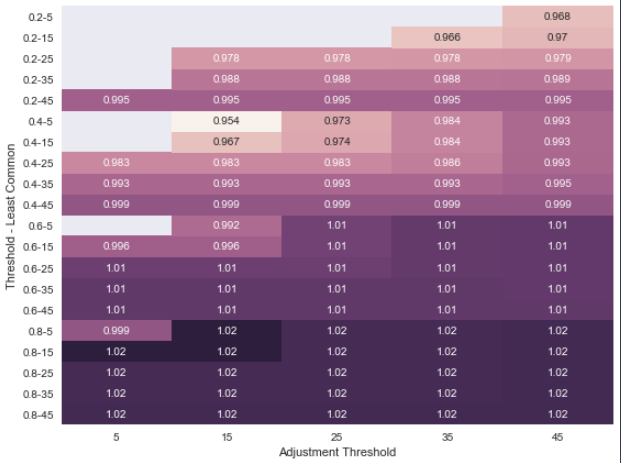
\includegraphics[width=1\textwidth]{../rmse}
    \caption{RMSE: experimental results}
    \label{fig:RMSE}
\end{figure}
 

Having the Pearson Correlation Matrix at hand, we use the following formula to make our predictions:

\[ P_{ik} = \bar{R_i}  + \frac{\sum{W_{ij}(R_{jk} - \bar{R_j})}}{\sum{W_{ij}}} \]

Firstly we tried to change the baseline estimation to incorporate the global average and the rating deviation of users and movies but we found that the user average produces better predictions.

The parameters we had to fine tune were the following: additionally to least  common rated movies and the correlation threshold we set the Adjustment Threshold to lower the significance of correlations based on few co-rated items. After running several experiments on parallel we produced the results shown on Figure \ref{fig:RMSE}. We found the our lowest value for RMSE is 0.9538 for threshold set to 0.4, least common items to 5 and a adjustment threshold at 15.

We tried using a negative threshold as well by taking the negative correlation values lower than it into account. We thought that extremely dissimilar users choices would lower the error, but that was not the case.
We also tried to use a Nearest Neighbors approach, but as shown on Figure \ref{fig:nnRMSE} the results were not improved and we the added sorting time was not justified. 

\begin{figure}[h]
    \centering
    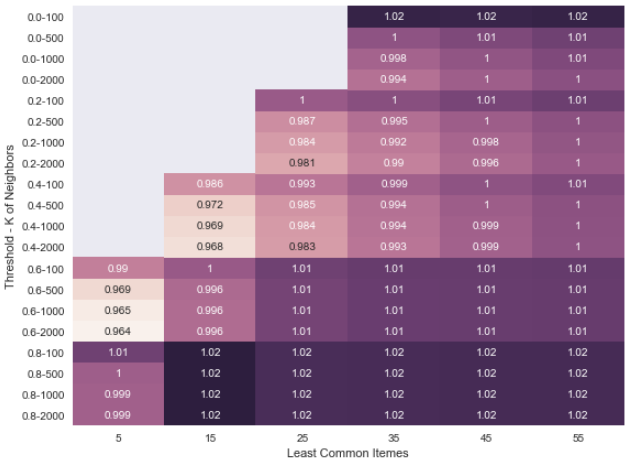
\includegraphics[width=1\textwidth]{../nnrmse}
    \caption{Nearest Neighbors RMSE: experimental results}
    \label{fig:nnRMSE}
\end{figure}

The memory limitation is the biggest constraint to our performance, the blank cells in our tables are the ones that we could not fit the Correlation Matrix in 2 Gigabytes of RAM. Closer we are to their configuration, the better the results we produced.

We have to note that the Pearson Correlation Matrix was produced with the Threshold Collaborating Filtering model in mind and not the kNN one. Thus, by only saving the most relevant users at the Matrix Computation phase we may could produce better results.

\end{document}

